\documentclass{exam}

\usepackage[spanish]{babel}
\usepackage[utf8]{inputenc}
\usepackage[T1]{fontenc}
\usepackage[newcommands]{ragged2e}
\usepackage{hyperref}
\usepackage{algorithm,algorithmic}
\usepackage{colortbl}
\usepackage{graphicx}
\usepackage{multicol}
\usepackage{enumitem}
\usepackage{float}
\usepackage{pdfpages}
\usepackage{
  amsmath,
  amssymb,
  eso-pic,
  float,
  graphicx,
  lmodern,
  wrapfig,
  tabularx,
  multicol,
  multirow,
  color,
  colortbl,
  lastpage,
  titlesec,
  sectsty
}


\definecolor{azul}{RGB}{33,127,190}
\sectionfont{\color{azul}}
\subsectionfont{\color{azul}}
\renewcommand{\familydefault}{\sfdefault}

\footer{}{\thepage}{}

\makeatother

\title{\LARGE\color{azul}\textbf{Estructura de Datos - Certamen 1 }}
\author{\smallsize \color{gray}{Profesor: } \color{black}{\textbf{Eduardo Godoy}}}
\date{\normalsize \em \today}

\begin{document}

\AddToShipoutPictureBG*{%
  \AtPageUpperLeft{\raisebox{-\height}{
\includegraphics[scale=.95]{base/header.png}}}}

\maketitle

\begin{multicols}{2}
  \begin{flushleft}
    \textbf{Nombre:} \\
    \vspace*{2mm}
    \textbf{Rut:} \\
    \vspace*{2mm}
    \textbf{Paralelo:}
  \end{flushleft}
  \begin{center}
    \begin{table}[H]
      \begin{tabular}{p{4cm}|p{3cm}|}
        \arrayrulecolor{gray!50}\cline{2-2} ~ & {\em {\scriptsize \color{gray!50}{Puntaje:}}}\\
         & ~ \\
         ~ & \textbf{Nota:}
        \\ & ~ \\
        \arrayrulecolor{gray!50}\cline{2-2}
      \end{tabular}
    \end{table}
  \end{center}
\end{multicols}

%\vspace*{-18mm}
\noindent
\textbf{\\Instrucciones:}
\begin{itemize}
\item[-] El puntaje máximo  es 100 puntos.
\item[-] Tiempo máximo: 120 minutos.
\item[-] El trabajo es \underline{\textbf{individual}}. Cualquier intento de copia, será sancionado según dicta el reglamento de la carrera.
\end{itemize}

\noindent
\textbf{Resultados de aprendizaje a evaluar:}
\begin{enumerate}
\item Conocer e Implementar algoritmos de ordenamiento y estructuras de datos complejas.
\vspace{2mm}

\noindent
\textbf{Contenido:} Este certamen evalúa los siguientes temas:

\vspace{-2mm}
\begin{table}[H]
  \begin{tabular}{
    !{\color{gray!50}\vrule}l
    !{\color{gray!50}\vrule}c
    !{\color{gray!50}\vrule}c
    !{\color{gray!50}\vrule}} \arrayrulecolor{gray!50} \hline
    \multicolumn{1}{!{\color{gray!50}\vrule}c}{\multirow{2}{*}{\textbf{
    Tema
    }}} &
          \multicolumn{2}{!{\color{gray!50}\vrule}c!{\color{gray!50}\vrule}}{\textbf{
          Puntajes
          }} \\ \arrayrulecolor{gray!50}\cline{2-3} &
                                                      \multicolumn{1}{!{\color{gray!50}\vrule}c!{\color{gray!50}\vrule}}{\textbf{
                                                      Total
                                                      }} &
                                                           \multicolumn{1}{c!{\color{gray!50}\vrule}}{\textbf{
                                                           Obtenido
                                                           }} \\ \arrayrulecolor{gray!50} \hline
    Problema 1: Complejidad de algoritmos
        & \multicolumn{1}{!{\color{gray!50}\vrule}c!{\color{gray!50}\vrule}}{\textbf{
          30 pts.
          }} & \\ \arrayrulecolor{gray!50} \hline
    Problema 2: Algoritmos de Ordenamientos
        & \multicolumn{1}{!{\color{gray!50}\vrule}c!{\color{gray!50}\vrule}}{\textbf{
          40 pts.
          }} & \\ \arrayrulecolor{gray!50} \hline
          Problema 3: TDA - Listas Enlazadas.
              & \multicolumn{1}{!{\color{gray!50}\vrule}c!{\color{gray!50}\vrule}}{\textbf{
                30 pts.
                }} & \\ \arrayrulecolor{gray!50} \hline

  \end{tabular}
\end{table}

\newpage

\vspace{-7mm}
\section{\textbf{Problema 1}}
\noindent
% \textbf{Plantamiento de problema: }
\begin{questions}
\item \textbf{\emph{30pts.}}

\begin{itemize}

    \item Analise los siguiente algoritmos y a continuación responda. \\


    \begin{tabular}{|p{40ex}|p{40ex}|}\hline
        $A_1:$ & $A_2:$ \\
        \texttt{\#include <stdio.h>}
                    & \texttt{\#include <stdio.h>} \\
        \texttt{int main()\{}
                    & \texttt{int main()\{} \\
        $~~$ \texttt{int n=100000; //$10^5$}
                    & $~~$ \texttt{int n=1000000; //$10^6$} \\
        $~~$ \texttt{int a[n];}
                    & $~~$ \texttt{int a[2*n];} \\
        $~~$ \texttt{for(int i=0; i<n; i++)\{}
                    & $~~$ \texttt{for(int i=0; i<2*n; i++)\{}\\
        $~~~~$ \texttt{a[i]=2*i;}
                    & $~~~~$ \texttt{a[i]=2*i;}\\
        $~~$ \texttt{\}} & $~~$ \texttt{\}}\\
        $~~$ \texttt{for(int i=0; i<n; i++)\{}
                    & $~~$ \texttt{return(0);}\\
        $~~~~$ \texttt{printf(``\%d tiene \%d$\backslash$n'',i,a[i]);} & \texttt{\}}\\
        $~~$ \texttt{\}} & \\
        $~~$ \texttt{return(0);} & \\
        \texttt{\}} & \\\hline
    \end{tabular}

    \begin{enumerate}
        \item ¿Cuántas veces itera cada uno de los tres ``\texttt{for}''? [5 pts]
        \item ¿Cómo calcula el tiempo de CPU de ejecución de cada algoritmo? Calcule. [10 pts]
        \item ¿Cuál es el tiempo de ejecución en notación big O de cada algoritmo? [10 pts]
        \item ¿Qué algoritmo es más eficiente en términos de complejidad temporal? [5 pts]
    \end{enumerate}
\end{itemize}

\begin{itemize}
    \item[$a)$] Los tiempos se deben sumar en notación big O.\tabto{82ex} [3 pts]\\
    El tiempo total será $2n^3+O(\frac{1}{2}n^2)=O(2n^3+\frac{1}{2}n^2)$,\tabto{82ex} [2 pts]\\
    es decir, $O(n^3)$.\tabto{82ex} [5 pts]
    \item[$b)$] Los tiempos se deben sumar en notación big O (o bien quedarme con el máximo).\tabto{82ex} [2 pts]\\
    El tiempo total será $2n^3+O(\frac{1}{2}n^2)+O(2^n)=O(2n^3+\frac{1}{2}n^2+2^n)$,\tabto{82ex} [2 pts]\\
    es decir, $O(2^n)$.\tabto{82ex} [6 pts]
    \item[$c)$] Calculos:
  \begin{enumerate}
    \item[$a)$] Cada \texttt{for} de $A_1$ itera $n=10^5$ veces. \tabto{82ex} [2 pts]\\
    El \texttt{for} de $A_2$ itera $2n=2\times10^6$ veces. \tabto{82ex} [3 pts]
    \item[$b)$] Puede variar entre cada máquina, pero debe ser el resultado \texttt{user} que retorna la ejecución con el comando \texttt{time}. \tabto{82ex} [5 pts]\\
    Escribir el resultado obtenido para $A_1$ y para $A_2$. \tabto{82ex} [5 pts]
    \item[$c)$] Para $A_1$ es $O(n+n)=O(2n)=O(n)$.\tabto{82ex} [5 pts]\\
  \end{enumerate}
    Para $A_2$ es $O(2n)=O(n)$.\tabto{82ex} [5 pts]
    \item[$d)$] De lo anterior se concluye que $A_1$ y $A_2$ tienen la misma complejidad temporal.\tabto{82ex} [5 pts]\\
\end{itemize}

\end{questions}

\begin{table}[H]
  \centering
  \begin{tabular}{
    !{\color{gray!50}\vrule}p{3.9cm}
    !{\color{gray!50}\vrule}p{3.6cm}
    !{\color{gray!50}\vrule}p{3.6cm}
    !{\color{gray!50}\vrule}p{3.6cm}
    !{\color{gray!50}\vrule}} \arrayrulecolor{gray!50} \hline
    \multicolumn{4}{!{\color{gray!50}\vrule}c!{\color{gray!50}\vrule}}{\textbf{¿Cómo  seré evaluado en este trabajo?}} \\ \arrayrulecolor{gray!50}
    \hline
    %
    \textbf{Ítem} & \textbf{Logrado} & \textbf{Suficiente} & \textbf{No Logrado}\\ \arrayrulecolor{gray!50} \hline\newline
    Pregunat 1. &
    Aplica de forma correcta: 5pts   &
    Aplica parcialmente con menos de 2 errores: 3pts  &
    Aplica de forma incorrecta con 3 errores o más: 0pts \\ \arrayrulecolor{gray!50} \hline

    Pregunat 2. &
    Aplica de forma correcta: 10pts   &
    Aplica parcialmente: 5pts  &
    Aplica de forma incorrecta: 0pts \\ \arrayrulecolor{gray!50} \hline

    Pregunat 3. &
    Aplica de forma correcta 10pts   &
    Aplica parcialmente 5pts &
    Aplica de forma incorrecta con 3 errores o más 0pts\\ \arrayrulecolor{gray!50} \hline

    Pregunta 4. &
    Aplica de forma correcta 5pts &
    Aplica parcialmente  3pts &
    Aplica de forma incorrecta  0pts\\ \arrayrulecolor{gray!50} \hline

    Total de la sección &  30pts & 15pts & 0pts\\ \arrayrulecolor{gray!50} \hline
  \end{tabular}
  \label{tbl:1}
\end{table}

\vspace{-5mm} \textbf{Nota:} En caso de que el ítem no esté presente,
tiene ponderación cero.



\newpage
\vspace{-7mm}
\section{\textbf{Problema 2}}
\noindent
% \textbf{Plantamiento de problema: }

\begin{questions}

  \begin{enumerate}
  \item \textbf{\emph{60pts.}} Utilizando la técnica del algoritmo Quick-Sort ordene el siguiente arreglo:

  \begin{table}[H]
  \centering
  \begin{tabular}{|l|l|l|l|l|l|l|l|l|l|}
  \hline
    8 & 5 & 2 & 6 & 8 & 3 & 1 & 4 & 0 & 7 \\
  \hline
  \end{tabular}
  \end{table}


\begin{itemize}
  \item Considere como criterio de selección del pivote el extremo el primero desde la izquierda.
\end{itemize}

    \end{enumerate}
    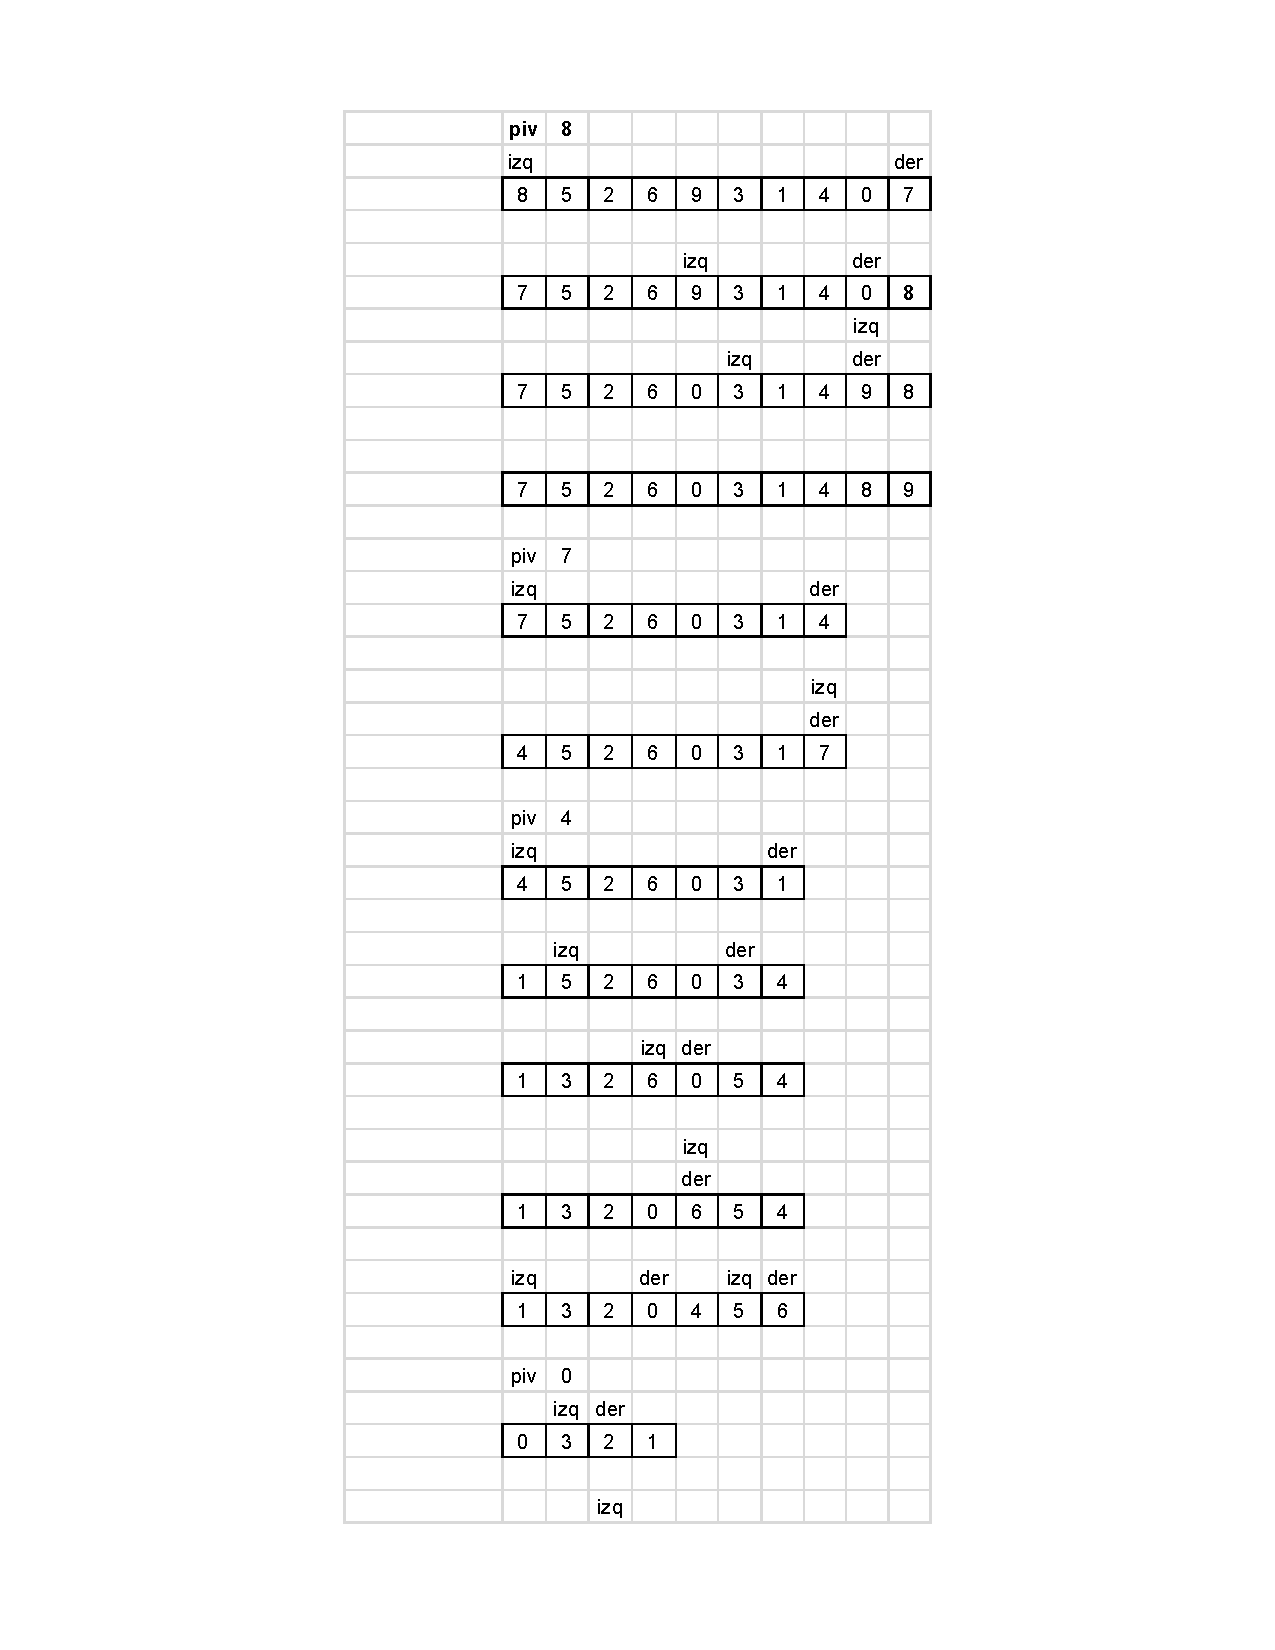
\includepdf[pages=1-2]{../image/cap2/ordenamientos_quicksort.pdf}
  \end{questions}

  \begin{table}[H]
    \centering
    \begin{tabular}{
      !{\color{gray!50}\vrule}p{3.9cm}
      !{\color{gray!50}\vrule}p{3.6cm}
      !{\color{gray!50}\vrule}p{3.6cm}
      !{\color{gray!50}\vrule}p{3.6cm}
      !{\color{gray!50}\vrule}} \arrayrulecolor{gray!50} \hline
      \multicolumn{4}{!{\color{gray!50}\vrule}c!{\color{gray!50}\vrule}}{\textbf{¿Cómo seré evaluado en este trabajo?}} \\ \arrayrulecolor{gray!50} \hline
      \textbf{Ítem} & \textbf{Logrado} & \textbf{Suficiente} & \textbf{No Logrado}\\ \arrayrulecolor{gray!50} \hline
      Conocimiento del algoritmo &
      Aplica de forma correcta 40 pts   &
      Aplica parcialmente con menos de 3 errores 20 pts  &
      Aplica de forma incorrecta con 3 errores o más 0pts\\ \arrayrulecolor{gray!50} \hline


      Total de la sección &  40pts & 20pts & 0pts\\ \arrayrulecolor{gray!50} \hline
    \end{tabular}
    \label{tbl:1}
  \end{table}
  \vspace{-5mm}
  \textbf{Nota:} En caso de que el {í}tem no est{é} presente, tiene ponderaci{ó}n cero.

  \newpage
  \vspace{-7mm}
  \section{\textbf{Problema 3}}
  \noindent
  \begin{questions}

    \begin{enumerate}
    \item \textbf{\emph{30pts.}}

    \item Considere el siguiente pseudocódigo, que define una lista doblemente enlazada de nodos:

    \texttt{struct Node \{}\\
    $~~~~$\texttt{data;} \tabto{23ex}// Dato almacenado en el nodo\\
    $~~~~$\texttt{next;} \tabto{23ex}// Puntero al nodo siguiente (NULL para el último nodo)\\
    \texttt{\}}\\
    \texttt{struct List \{}\\
    $~~~~$\texttt{Node FirstNode;} \tabto{23ex}// La lista apunta al primer nodo; NULL si está vacía\\
    $~~~~$\texttt{Node LastNode;} \tabto{23ex}// La lista apunta al último nodo; NULL si está vacía\\
    \texttt{\}}

    Para insertar un nodo \texttt{newNode} después de un nodo \texttt{node}, se define la función \texttt{insertAfter}:

    \texttt{function insertAfter(Node node, Node newNode) \{}\\
    $~~~~$\texttt{newNode.next := node.next;}\\
    $~~~~$\texttt{node.next := newNode;}\\
    \texttt{\}}

    Para insertar un nodo \texttt{newNode} al inicio de la lista \texttt{list}, se define la función \texttt{insertBeginning}:

    \texttt{function insertBeginning(List list, Node newNode) \{}\\
    $~~~~$\texttt{newNode.next   := list.firstNode;}\\
    $~~~~$\texttt{list.firstNode := newNode;}\\
    \texttt{\}}

    A partir de lo anterior, defina:
    \begin{enumerate}
        \item Una función \texttt{insertEnd}, que inserta un nodo \texttt{newNode} al final de \texttt{list}. \tabto{76ex} [15 pts]
        \item Una función \texttt{removeAfter}, que elimina un nodo \texttt{Node}. \tabto{76ex} [15 pts]
    \end{enumerate}
\end{enumerate}

      \end{enumerate}


      \begin{enumerate}

          \item[$a)$] La función queda definida por:\\[1.2ex]
          \texttt{function insertEnd(List list, Node newNode) \{}\\
          $~~~~$\texttt{(list.LastNode).next := newNode;}\\
          \texttt{\}} \tabto{81ex} [15 pts]
          \item[$b)$] La función queda definida por:\\[1.2ex]
          \texttt{function removeAfter(Node node) \{}\\
          $~~~~$\texttt{aux := node.next;}\\
          $~~~~$\texttt{node.next := node.next.next;}\\
          $~~~~$\texttt{destroy aux;}\\
          \texttt{\}} \tabto{81ex} [15 pts]
      \end{enumerate}
    \end{questions}


    \begin{table}[H]
      \centering
      \begin{tabular}{
        !{\color{gray!50}\vrule}p{3.9cm}
        !{\color{gray!50}\vrule}p{3.6cm}
        !{\color{gray!50}\vrule}p{3.6cm}
        !{\color{gray!50}\vrule}p{3.6cm}
        !{\color{gray!50}\vrule}} \arrayrulecolor{gray!50} \hline
        \multicolumn{4}{!{\color{gray!50}\vrule}c!{\color{gray!50}\vrule}}{\textbf{¿Cómo seré evaluado en este trabajo?}} \\ \arrayrulecolor{gray!50} \hline
        \textbf{Ítem} & \textbf{Logrado} & \textbf{Suficiente} & \textbf{No Logrado}\\ \arrayrulecolor{gray!50} \hline
        \textbf{insertEnd}. &
        Aplica de forma correcta 15pts   &
        Aplica parcialmente  7 errores 5pts  &
        Aplica de forma incorrecta 0pts\\ \arrayrulecolor{gray!50} \hline

        \textbf{removeAfter}. &
        Aplica de forma correcta 15pts   &
        Aplica parcialmente  3pts  &
        Aplica de forma incorrecta 0pts\\ \arrayrulecolor{gray!50} \hline


        Total de la sección &  60pts & 30pts & 0pts\\ \arrayrulecolor{gray!50} \hline
      \end{tabular}
      \label{tbl:1}
    \end{table}
    \vspace{-5mm}
    \textbf{Nota:} En caso de que el {í}tem no est{é} presente, tiene ponderaci{ó}n cero.
\end{document}
